\paragraph{Example of infinite expectation}
$$P(X = 2^n) = 2^{-n}$$
The model is flipping coin until you get head and getting $2^n$ dollars where $n$ is number of flips you made.
Then expectancy of your profit
$$EX = \sum 2^n 2^{-n} = \infty$$

\section{ Continuous random variables}
Since $f(x) = F^\prime(x)$
$$\int_{-\infty}^{\infty} f(x) dx = 1$$
We define expectation of $X$ as
$$\mu = \mathbb{E}X = \int_{-\infty}^{\infty} xf(x) dx$$
We can define expectation in broad sense. If one of $\int_{-\infty}^0 xf(x) dx$ and $\int_0^\infty xf(x) dx$ is finite and second is infinite, we can define expectation as infinite.

 \subsection{Function of continuous of random variable}
 For $X: \Omega \to \mathbb{R}$ define 
 $$Y = \Psi(X)$$
 Then
 $$\mathbb{E}Y = \mathbb{E} \Psi(X) = \int_{-\infty}^\infty = \int_{-\infty}^\infty \Psi(x) f(x) dx$$
Now we can use it to define variance, by using $\psi(x) = (x-\mu)^2$:
$$\sigma^2 = \mathbb{E}(X-\mu)^2 = \int_{-\infty}^\infty (x-\mu)^2 f(x)dx$$

\paragraph{Claim}
$$\sigma^2(X) = \mathbb{E}X^2 - (\mathbb{E}X)^2$$
\subparagraph{Proof}
$$\sigma^2(X) = \int_{-\infty}^\infty  (x-\mu)^2 f(x) dx =\int_{-\infty}^\infty x^2 f(x) dx-2\mu \int_{-\infty}^\infty  \underbrace{x f(x)}_{\mu} dx+\mu^2\underbrace{\int_{-\infty}^\infty  f(x) dx}_{1} = EX^2-\mu^2$$

\subsection{Classical continuous distributions}
\subsubsection{Uniform distribution}
For $[a,b]$:
$$f(x) = \begin{cases}
\frac{1}{b-a}&  a \leq x\leq b\\0& otherwise
\end{cases}$$

$$EX = \frac{b+a}{2}$$
We write $X \sim U\big( [a,b] \big)$.

\begin{center}	
	\includesvg[eps,svgpath = lect9/,width=0.5\linewidth]{uniform}
\end{center}
\subsubsection{Exponential distribution}
For $\lambda > 0$
$$f(x) = \lambda e^{-\lambda x}, \: x \geq 0$$
Then $$F(x) = \int_{-\infty}^x f(t) dt = \int_0^x f(x) dt = 1-e^{-\lambda x}$$
$$EX = \int_0^\infty x \lambda e^{-\lambda x} dx = \left[ -xe^{-\lambda x} \right]_0^\infty + \int_0^\infty e^{-\lambda x}dx = \frac{1}{\lambda }$$
$$\sigma^2 = EX^2 - (EX)^2 = EX^2 - \left(\frac{1}{\lambda}\right)^2 = \frac{1}{\lambda^2} $$

\begin{center}	
	\includesvg[eps,svgpath = lect9/,width=0.5\linewidth]{exp}
\end{center}

If $X \sim Exp(\lambda)$ then 
$$P(X \geq a+b | X\geq a) = P(X \geq b)$$
This property is called memorylessness.
\paragraph{Proof that exponential distribution is memoryless}
$$P(X \geq a+b | X \geq a)= \frac{P(X \geq a+b, \: X \geq a)}{P(X \geq a)}= \frac{P(X \geq a+b) }{P(X \geq a)} = \frac{e^{-\lambda(a+b)}}{e^{-\lambda a}}=e^{-\lambda b}$$ 
\paragraph{Notation}
$P(A,B) = P(A \cap B)$
\paragraph{Model}
For example, the time until a radioactive particle decays or time until you get cellphone call.


\subsubsection{Normal (Gaussian) distribution}
\paragraph{Proof of integral}
Denote $$l =  \int_{-\infty}^\infty  e^{-\frac{x^2}{2}}dx$$
Since $l$ is even;
$$\frac{l}{2} =  \int_{0}^\infty  e^{-\frac{x^2}{2}}dx$$
Now
$$\frac{l^2}{4} =  \int_{0}^\infty  e^{-\frac{x^2}{2}}dx\int_{0}^\infty  e^{-\frac{y^2}{2}}dy = \int_{0}^\infty \int_{0}^\infty  e^{-\frac{x^2+y^2}{2}}dxdy$$
The integral is in first quarter. Switching to polar:
$$dxdy = rdr d\theta$$
$$\frac{l^2}{4}  = \int_{0}^\infty \int_{0}^\infty  e^{-\frac{x^2+y^2}{2}}dxdy = \int_0^\frac{\pi}{2} d\theta \int_0^\infty dr re^{-\frac{r^2}{2}} =  \int_0^\frac{\pi}{2} d\theta \left[ -e^{-\frac{r^2}{2}} \right]_0^\infty =  \int_0^\frac{\pi}{2} = \frac{\pi}{2}$$
$l = \sqrt{2\pi}$
\paragraph{Normal distribution}
$$f(x) = c e^{-\frac{(x-a)^2}{2b}}$$
$$\int_{-\infty}^\infty f(x) = c \int_{-\infty}^\infty  e^{-\frac{(x-a)^2}{2b}} = 1$$
Substitute $z = \frac{x-a}{\sqrt{b}}$ and $dx = \sqrt{b}dz$.

$$c \int_{-\infty}^\infty  e^{-\frac{(x-a)^2}{2b}} = c\sqrt{b} \int_{-\infty}^\infty  e^{-\frac{z^2}{2}}dz c\sqrt{2\pi b}$$
Then
$$c = \frac{1}{\sqrt{2\pi b}}$$
and
$$f(x) = \frac{1}{\sqrt{2\pi b}} e^{-\frac{(x-a)^2}{2b}}$$
which is density function.
\paragraph{Expectation of normal distribution}
$$\int_{-\infty}^\infty x f(x) dx = \int_{-\infty}^\infty x f(x)\frac{e^{-\frac{(x-a)^2}{2b}}}{\sqrt{2\pi b}}  dx =  \underbrace{\int_{-\infty}^\infty (x-a) f(x)\frac{e^{-\frac{(x-a)^2}{2b}}}{\sqrt{2\pi b}}  dx}_{\text{odd function} \Rightarrow =0} + \int_{-\infty}^\infty a f(x)\frac{e^{-\frac{(x-a)^2}{2b}}}{\sqrt{2\pi b}}  dx = a\int_{-\infty}^\infty  f(x)\frac{e^{-\frac{(x-a)^2}{2b}}}{\sqrt{2\pi b}}  dx = a$$
Since $a$ is mean, we'll replace it with $\mu$:
$$f(x) = \frac{e^{-\frac{(x-\mu)^2}{2b}}}{\sqrt{2\pi b}} $$


\paragraph{Variance of normal distribution}
$$\int_{-\infty}^\infty z^2 e^{-\frac{z^2}{2}} dz $$
By parts: $u=z$ and $v^\prime = ze^{-\frac{z^2}{2}}$. Then
$$\int_{-\infty}^\infty z^2 e^{-\frac{z^2}{2}} dz = \left[ -z  e^{-\frac{z^2}{2}} \right]_{-\infty}^\infty + \int_{-\infty}^\infty e^{-\frac{z^2}{2}} dz = \sqrt{2 \pi}$$
lets calculate variance:
$$\sigma^2 = \int_{-\infty}^\infty (x-\mu)^2 \frac{e^{-\frac{(x-\mu)^2}{2b}}}{\sqrt{2\pi b}} dx$$
With same substitution  $z = \frac{x-\mu}{\sqrt{b}}$:
$$\sigma^2 = \int_{-\infty}^\infty bz^2 \frac{e^{-\frac{z^2}{2}}}{\sqrt{2\pi}} dz =b \underbrace{\int_{-\infty}^\infty z^2 \frac{e^{-\frac{z^2}{2}}}{\sqrt{2\pi}} dz}_{1} = b $$
Thus $\sqrt{b} = \sigma$.

Which leads us to final form of $f(x)$:
$$f(x) = \frac{e^{-\frac{(x-\mu)^2}{2\sigma^2}}}{\sqrt{2\pi}\sigma} $$
We write $X \sim N(\mu, \sigma^2)$.

\begin{center}	
	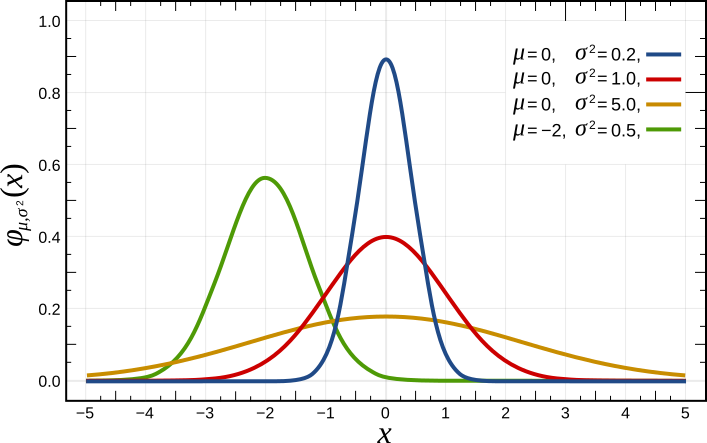
\includegraphics[width=0.5\linewidth]{./lect9/norm.png}
\end{center}